\documentclass[tikz]{standalone}

\usepackage{tikz}
\usetikzlibrary{shapes.arrows, fadings}

\begin{document}
    \begin{tikzpicture}
        \node (generality_arrow) at (0, 0) [
            draw=black,
            left color=white,
            single arrow,
            right color=red,
            single arrow,
            minimum height=11cm,
            shading angle=90+270,
            rotate=270
        ] {};
        \path (generality_arrow.south) + (0, -5.5) node[anchor=north] (generality) {\textcolor{red}{Generality}};
        \path (generality_arrow) + (1, 0) node (compactness_arrow) [
            draw=black,
            left color=white,
            single arrow,
            right color=blue,
            single arrow,
            minimum height=11cm,
            shading angle=90+90,
            rotate=90
        ] {};
        \path (compactness_arrow.north) + (0, 5.5) node[anchor=south] (generality) {\textcolor{blue}{Compaction}};

        \path (generality_arrow) + (-10, 5) node (manhattan) {\large Manhattan world};
        \path (manhattan.south west) node[anchor=north west, text width=7cm] (manhattan_cite) {\small \parencite{vanegas2010building},~\parencite{li2016manhattan}};
        \path (manhattan_cite.east) + (2, 0) node[anchor=west] (manhattan_image) {
            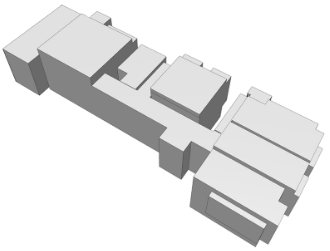
\includegraphics[width=2cm]{images/modeling_approaches/boxfitting_li}
        };
        \path (manhattan_cite.south west) + (0, -.5) node[anchor=north west] (piecewise) {\large Piecewise planar structures};
        \path (piecewise.south west) node[anchor=north west, text width=7cm] (piecewise_cite) {\small \parencite{lafarge_ijcv12},~\parencite{nan2017polyfit}};
        \path (piecewise_cite.east) + (2, 0) node[anchor=west] (piecewise_image) {
            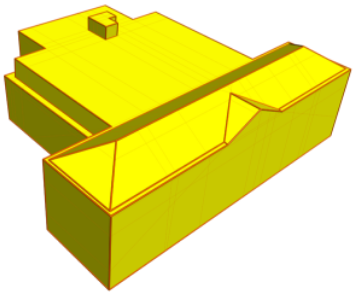
\includegraphics[width=2cm]{images/modeling_approaches/polyfit_iccv}
        };
        \path (piecewise_cite.south west) + (0, -.5) node[anchor=north west] (grammar) {\large Grammar based};
        \path (grammar.south west) node[anchor=north west, text width=7cm] (grammar_cite) {\small \parencite{nan2015template},~\parencite{zeng2018neural}};
        \path (grammar_cite.east) + (2, 0) node[anchor=west] (grammar_image) {
            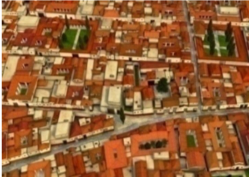
\includegraphics[width=2cm]{images/modeling_approaches/grammar}
        };
        \path (grammar_cite.south west) + (0, -.5) node[anchor=north west] (simplification) {\large Mesh simplification};
        \path (simplification.south west) node[anchor=north west, text width=7cm] (simplification_cite) {\small \parencite{zhou20102},~\parencite{verdie2015lod}};
        \path (simplification_cite.east) + (2, 0) node[anchor=west] (simplification_image) {
            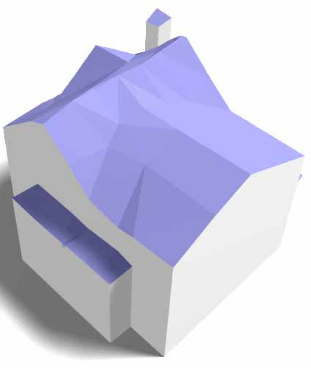
\includegraphics[width=2cm]{images/modeling_approaches/dual_zhou}
        };
    \end{tikzpicture}
\end{document}
